\documentclass[tikz,border=10pt]{standalone}
\usetikzlibrary{arrows.meta, decorations.pathreplacing}

\begin{document}

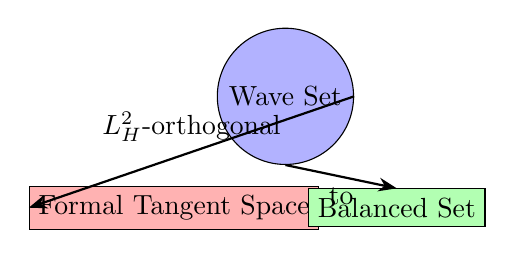
\begin{tikzpicture}[node distance=2cm]

    % Nodes
    \node (wave_set) [circle, draw, fill=blue!30] {Wave Set};
    \node (formal_tangent_space) [rectangle, draw, fill=red!30, below left of=wave_set] {Formal Tangent Space};
    \node (balanced_set) [rectangle, draw, fill=green!30, below right of=wave_set] {Balanced Set};

    % Arrows
    \draw[-Stealth, thick] (wave_set.east) -- node[midway, above] {$L^2_H$-orthogonal} (formal_tangent_space.west);
    \draw[-Stealth, thick] (wave_set.south) -- node[midway, below] {to} (balanced_set.north);

\end{tikzpicture}

\end{document}